\chapter{Aufgabe 5: Heated Plate Parallel}

Die Abbildungen in~\ref{fig:aufgabe5} visualisiert das Laufzeitverhalten beim Erhöhen der Threads und die Tabelle~\ref{tab:aufgabe5} listet die Laufzeiten auf. Die Laufzeit wird immer niedriger bis einschließlich 16 Threads. Da maximal 16 Kerne verfügbar waren (Einstellung in der Job-Datei), handelt es sich bei der Ausführung mit 32 Threads nicht tatsächlich um eine parallele Ausführung mit einem Team von 32 Threads. Vermutlich werden in diesem Fall einige Tasks sequentiell ausgeführt oder in besonderer Weise gescheduled, was einen zusätzlichen Overhead verursacht, der die Laufzeit extrem erhöht.

In Abb.~\ref{fig:aufgabe5_logplot}, in dem die Laufzeit doppellogarithmisch über die Anzahl paralleler Threads aufgetragen wurde, lässt sich ablesen, dass die Laufzeit etwa mit linearer Ordnung mit der Anzahl paralleler Threads sinkt.

\begin{figure}[htbp]
 \centering 
 \begin{subfigure}{.49\textwidth}
  \centering 
  \includegraphics[width=1\textwidth]{img/aufgabe5_barplot.eps}
  \caption{Säulendiagramm.}
  \label{fig:aufgabe5_barplot}
 \end{subfigure}
%
 \begin{subfigure}{.49\textwidth}
  \centering 
  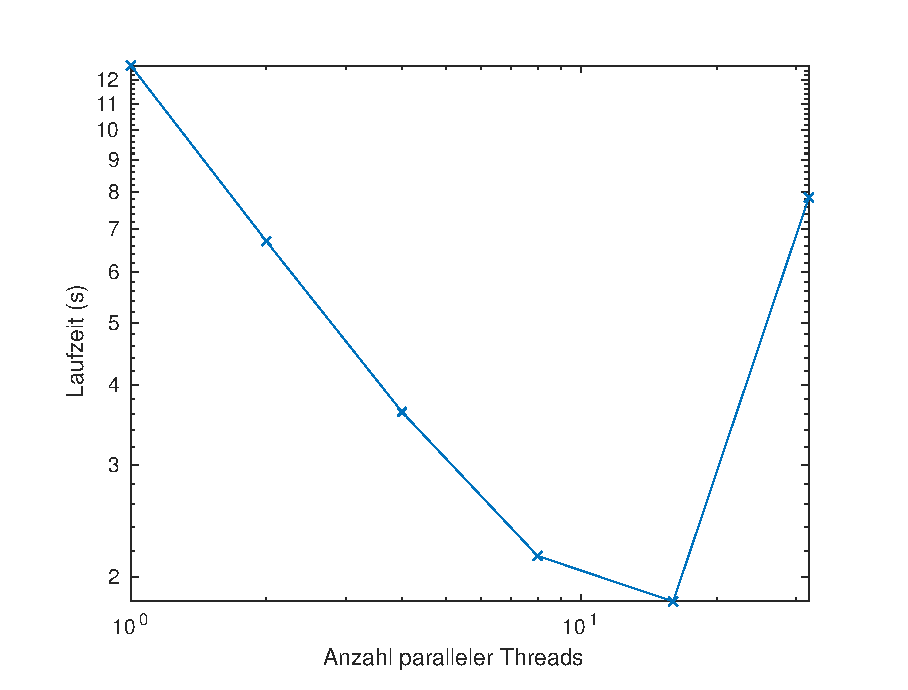
\includegraphics[width=1\textwidth]{img/aufgabe5_logplot.eps}
  \caption{Doppellogarithmische Darstellung.}
  \label{fig:aufgabe5_logplot}
 \end{subfigure}
\caption{Laufzeiten für sequentielle Ausführung und parallele Ausführung mit 1, 2, 4, 8, 16, 32 Threads von heated-plate-parallel.}
\label{fig:aufgabe5}
\end{figure}

\begin{table}[htbp]
 \centering 
 \caption{Laufzeiten für heated-plate-parallel.}
 \begin{tabular}{|l|r|}
  \textbf{Anzahl Threads} & \textbf{Laufzeit (s)} \\ \hline 
  1 & 12.6293 \\
  2 & 6.7073 \\
  4 & 3.6273 \\
  8 & 2.1598 \\
  16 & 1.8332 \\
  32 (16) & 7.8544
 \end{tabular}
\label{tab:aufgabe5}
\end{table}
